\documentclass[]{article}
\usepackage{mathrsfs}
\usepackage{amsmath}
\usepackage{amsfonts}
\usepackage{graphicx}
\usepackage[left=20mm, right=20mm, top=20mm, bottom=20mm]{geometry}


\begin{document}
\huge Transformada de Laplace.
\\

\normalsize Para comenzar a entender la transformada de Laplace debemos tener en claro como funciona la transformada de Fourier. Recordemos la definición.
\\
La transformada de Fourier de una función $f(t)$ se define:
$$
F(\omega) = \int_{-\infty}^{\infty}f(t)e^{-i\omega t} dt 
$$
\\
La transformada de Fourier venía acompañada de una condición necesaria que decía que $f(t)$ debe ser seccionalmente continua y de módulo integrable en todo el eje real, por ello muchas funciones no eran transformables ya que el area encerrada bajo la curva de estás tendería a infinito cuando $t\rightarrow \infty$.

Para solucionar esto, es conveniente multiplicar por un factor exponencial decreciente $e^{-\alpha t }$ obteniendose:
$$
\int_{-\infty}^{\infty} f(t) \cdot  e^{-\alpha t}\cdot  e^{-i\omega t}dt =
\int_{-\infty}^{\infty} f(t) \cdot  e^{-st}
$$
con $s=\alpha + i \hspace{3pt} \omega $
\\ Y esta es la definición de la transformada de Laplace. Esta, al igual que la transformada de Fourier se aplica en el dominio del tiempo, pero nos devuelve una funcion en un dominio de vairable compleja $s$ que llamaremos dominio de Laplace.
\\ Dentro del enfoque de la materia se trabajará con la versión unilateral de la transformada bajo la supocisión que todas las funciones $f(t)$ trabajadas cumpliran 
$f(t) = 0  \hspace{10pt} \forall t < 0$.
$$
F(s) = \int_{0}^{\infty} f(t) e^{-st} dt
$$
\\
\\
\Large Teorema de existencia.
\\

\normalsize Sea $f(t)$ una función seccionalmente continua y $f(t)$ de orden exponencial $\gamma$ para $t > N \Rightarrow \exists \hspace{5pt} \mathscr{L}[f(t)]$

Una función $f(t)$ es de orden exponencial $\gamma \Longleftrightarrow$ ${\exists \hspace{5pt} M,\gamma \in \mathbb{R}  / \forall t > N: |e^{-\gamma t} f(t)| < M }$ si $t \rightarrow \infty$.

Es decir, la función en módulo no puede crecer mas que $Me^{\gamma t}$ a partir de un cierto valor $N$.


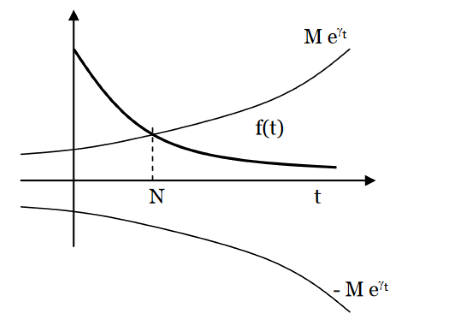
\includegraphics{../../../Imagenes/Superior/TransformadaDeLaplace/Laplace01.PNG}
\\
\\
\Large Propiedades de la transformada de Laplace
\normalsize
\\
\\
$a)$ Linealidad
$$
F(s) = \mathscr{L}[f(t)]\hspace{7pt} \wedge\hspace{7pt} G(s) = \mathscr{L}[g(t)]\hspace{7pt} \wedge\hspace{7pt} k_{1} , k_{2} \in \mathbb{R} \Rightarrow \mathscr{L}[k_{1}f(t) + k_{2}g(t)] = k_{1} F(s) + k_{2} G(s)
$$
\\
\\
$b)$ Primera propiedad de traslación

$$
F(s) = \mathscr{L}[f(t)] \Rightarrow \mathscr{L}[e^{at}f(t)] = F(s-a)
$$
Esto significa que multiplicar por $e^{at}$ en el dominio del tiempo, equivale a efectuar una traslación de $a$ unidades hacia la derecha en el dominio de Laplace.
\\
\\
$c)$ Segunda propiedad de traslación

$$
F(s) = \mathscr{L}[f(t)] \hspace{5pt} \wedge \hspace{5pt} g(t) = \left\{
	\begin{array}{ll}
		f(t-a) \hspace{10pt} t > a \\
		0 \hspace{40pt} t < a
	\end{array}
\right. \\
\Rightarrow \mathscr{L}[g(t)] = e^{-as}F(s)
$$

Esto significa que una traslación de $a$ unidades hacia la derecha en el dominio del tiempo equivale a multiplicar por $e^{-as}$ en el dominio de Laplace.
\\
\\
$d)$ Cambio de escala
$$
F(s) = \mathscr{L}[f(t)] \Rightarrow \mathscr{L}[f(at)] = \frac{1}{a}F(\frac{s}{a})	
$$
\\
\\
$e)$ Transformada de las derivadas

$$
F(s) = \mathscr{L}[f(t)] \Rightarrow \mathscr{L}[f^{n}(t)] = s^{n}\cdot F(s) -s^{n-1}f(0) - s^{n-2} f'(0) - \dots - f^{n-1}(0)
$$
Se puede encontrar una relación entre esta propiedad y el binomio de Newton. Al avanzar en la sumatoria (de restas) el grado de $s^{n}$ va decreciendo mientras que el "grado" (orden) de la derivada de $f(0)$ va aumentando.\\
Además vale la pena observar que una derivada en el dominio del tiempo, se traduce a un polinomio en el dominio de Laplace, esto junto con la propiedad siguiente será muy util para resolver ecuaciones diferenciales e integrodiferenciales.
\\
\\
$f)$ Transformada de la integral simple

$$
F(s) = \mathscr{L}[f(t)] \Rightarrow \mathscr{L}[\int_{0}^{t}f(u)du] = \frac{F(s)}{s}
$$
\\
\\
$g)$ Multiplicación por $t^{n}$

$$
F(s) = \mathscr{L}[f(t)] \Rightarrow \mathscr{L}[t^{n}f(t)] = (-1)^{n}F^{(n)}(s)
$$
Es decir, multiplicar por $t^{n}$	en el dominio del tiempo equivale a derivar en el orden $n$ en el dominio de Laplace.
\\
\\
$h)$ División por $t$

$$
F(s) = \mathscr{L}[f(t)] \Rightarrow \mathscr{L}[\frac{f(t)}{t}] = \int_{s}^{\infty}F(u)du
$$
Esto es valido siempre que $\exists \lim_{t\rightarrow 0} \frac{f(t)}{t}$
Es decir, dividir por $t$ en el dominio del tiempo, equivale a integrar en el dominio de Laplace. Observar que en el dominio de Laplace tenemos una función integral, al resolver nos quedará una función de $s$ como cualquier otra transformada.
\\
\\
$i)$ Teorema del valor inicial

Si existen los limites indicados, se cumple:

$$
\lim_{t\rightarrow 0} f(t) = \lim_{s\rightarrow \infty} sF(s)
$$
\\
\\
$j)$ Teorema del valor final

$$
\lim_{t\rightarrow \infty} f(t) = \lim_{s\rightarrow 0} sF(s)
$$

Observar que en estas ultimas dos propiedades la transformada está multiplicada por $s$
\\
\\
$k)$ Transformada de funciones periódicas
4
$$
f(t) = f(t+T) \Rightarrow F(s) = \mathscr{L}[f(t)] = \frac{1}{1-e^{-sT}}\int_{0}^{T}e^{-st}f(t)dt
$$
\\
\\
\Large Funciones utiles
\normalsize
\\

Estas son algunas funciones muy elementales y nos serán utiles para calcular transformadas de Laplace sin tener que usar la definición. Nos basaremos en estas funciones y haremos todos los calculos teniendo en cuenta las propiedades detalladas anteriormente.

\Large
$$
\setlength{\tabcolsep}{20pt}
\renewcommand{\arraystretch}{1.5}
\begin{tabular}{|c|c|}
	\hline
	\textbf{$f(t)$} & \textbf{$\mathscr{L}[f(t)] = F(s)$}\\
	\hline
	
	$1$ & $\frac{1}{s}$ \\

	\hline
	$t$ & $\frac{1}{s^{2}}$ \\
	\hline
	$t^{n}$ & $\frac{n!}{s^{n+1}}$ \\
	\hline
	$e^{at}$ & $\frac{1}{s-a}$ \\
	\hline
	$\sin{at}$ & $\frac{a}{s^{2}+a^{2}}$ \\
	\hline
	$\cos{at}$ & $\frac{s}{s^{2}+a^{2}}$ \\
	\hline
	$\delta(t)$ & $1$ \\
	\hline
\end{tabular}
$$

\normalsize
La función $\delta(t)$ es una funcíon especial y será explicada mas adelante.
\\
\\
\Large Funciones especiales.
\normalsize
\\

Son funciones muy utilizadas dentro de la ingenieria y nos permiten modelar ciertos sistemas comunes. Además nos facilitaran el calculo de ciertas transformadas.
\\
\\
\Large Función escalón unitario

\normalsize


$$
E(t) = \left\{
	\begin{array}{ll}
		1 \hspace{10pt} t > 0 \\
		0 \hspace{10pt} t < 0
	\end{array}
\right. \\
$$
o bien
$$
E(t-a) = \left\{
	\begin{array}{ll}
		1 \hspace{10pt} t > 0 \\
		0 \hspace{10pt} t < a
	\end{array}
\right. \\
$$
\\
Esta función es muy importante, ya que multiplicada por una constante, puede representar funciones constantes apartir de un cierto instante $a$. Es muy util para representar una señal de tensión continua, o una fuerza constante aplicada sobre algún sistema mecánico.

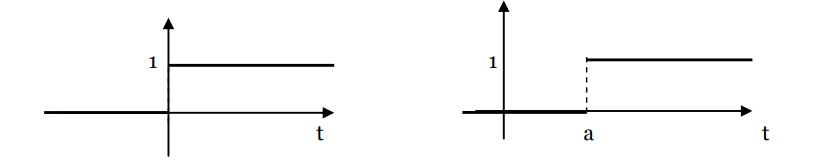
\includegraphics{../../../Imagenes/Superior/TransformadaDeLaplace/Laplace02.PNG}

La trasnformada de $E(t)$ aparece en la tabla y la de $E(t-a)$ es muy sencilla de calcular con la segunda propiedad de traslación.
$$
\mathscr{L}[E(t)] = \frac{1}{s}
$$
$$
\mathscr{L}[E(t-a)] = \frac{e^{-as}}{s}
$$

Además la función $E(t-a)$ resulta muy util para considerar funciones a partir de un cierto instante y definir funciones por trozos.
Consideremos el siguiente ejemplo:

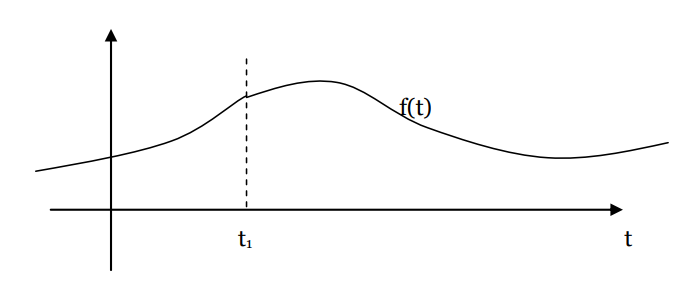
\includegraphics{../../../Imagenes/Superior/TransformadaDeLaplace/Laplace03.PNG}


Si multiplicamos $f(t)$ por $E(t-t_{1})$ obtenemos: 

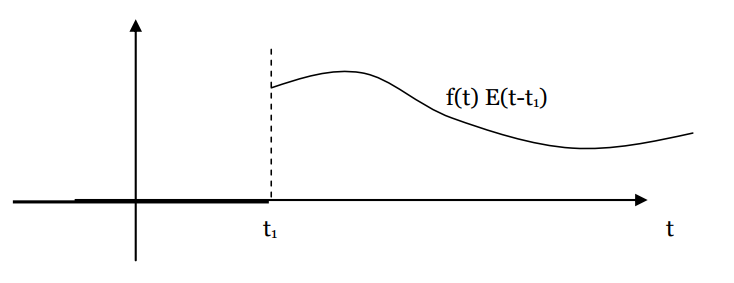
\includegraphics{../../../Imagenes/Superior/TransformadaDeLaplace/Laplace04.PNG}

Como $E(t-t_{1})$ vale $0$ antes de $t_{1}$ al multiplicar por $f(t)$ esta se reduce a $0$, y despues de $t_{1}$ la funcion $f(t)$ queda igual porque se está multiplicando por $1$.

Veamos ahora un ejemplo aún mas util que nos facilitará el calculo de una transformada. Como ya mencionamos, la funcíon $E(t)$ nos ayuda a la hora de escribir funciones por partes y ciertamente nos ayudará a calcular su transformada.

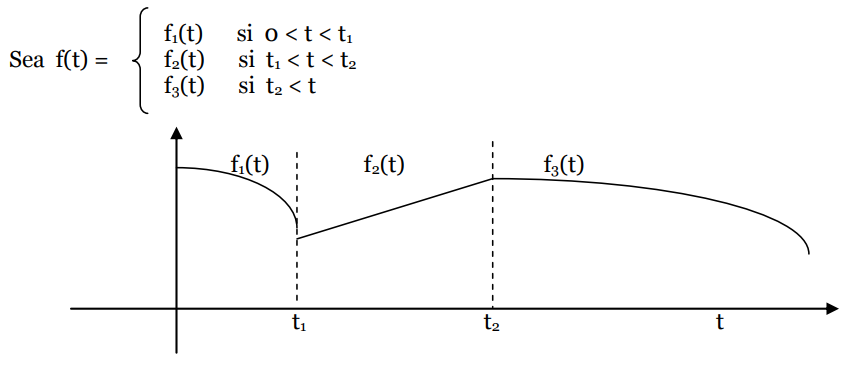
\includegraphics{../../../Imagenes/Superior/TransformadaDeLaplace/Laplace05.PNG}


Entonces $f(t)$ puede ser escrita de la siguiente forma.
$$
f(t) = f_{1}(t)\cdot (E(t)-E(t-t_{1})) + f_{2}(t) \cdot (E(t-t_{1})-E(t-t_{2})) + f_{3}(t)E(t-t_{2})
$$
Simplificaremos la notación para resolver los calculos mas facil llamando:
\begin{align}
	E(t) &= E_{0} \\
	E(t-t_{n}) &= E_{t_n} 
\end{align}
Entonces se deduce:
\begin{align}
  f(t) &= f_{1}(t)\cdot (E_0-E_{t_1}) + f_{2}(t) \cdot (E_{t_1}-E_{t_2}) + f_{3}(t)E_{t_2} \\
	f(t) &= f_1(t)E_{0} - f_1(t)E_{t_{1}} + f_2(t)E_{t_{1}} - f_2(t)E_{t_2} +f_3(t)E_{t_2} \\
	f(t) & = f_1(t)E_0 + E_{t_1}\cdot(f_2(t) - f_1(t)) + E_{t_2}\cdot(f_3(t)-f_2(t))
\end{align}
Al aplicar la transformada queda:
\begin{align}
  F(s) &= \mathscr{L}[f_1(t)E_0 + E_{t_1}\cdot(f_2(t) - f_1(t)) + E_{t_2}\cdot(f_3(t)-f_2(t))] \\
  F(s) &= \mathscr{L}[f_1(t)E_0] + \mathscr{L}[E_{t_1}\cdot(f_2(t) - f_1(t))] + \mathscr{L}[ E_{t_2}\cdot(f_3(t)-f_2(t))] \\
  F(s)& = \mathscr{L}[f_1(t)] + e^{-t_1s}\cdot (\mathscr{L}[f_2(t+t_1)] - \mathscr{L}[f_1(t+t_1)]) + e^{-t_2s} \cdot(\mathscr{L}[f_3(t+t_2)]-\mathscr{L}[f_2(t+t_2)]) 
\end{align}
\\
Cabe observar que en el ultimo paso las $f_n$ aparecen aplicadas en $t+t_n$, esto se debe a que, aplicar la transformada a una funcíon multiplicada por un escalón $E_{t_n}$ es equivalente a aplicar la transformada a la funcíon corrida hacia el eje de ordenadas $t_n$ unidades y multiplicar por el factor $e^{-t_n s}$. Para ver esto mas claro podemos pensar en la segunda propiedad de traslación, donde la $g(t)$ es nuestra $f_n(t)$ y la $f(t)$ es nuestra $f_n(t+t_n)$. Luego, la transformada se separa en dos por linealidad. 
\\
\\
\Large Función impulso unitario
\\
\normalsize
Es una función muy util para representar un valor en un lapso de tiempo infinitesimal, por ejemplo una fuerza aplicada en un instante dado a un bloque de masa. Esta descripción nos puede llevar a pensar si en verdad se trata de una función, lo discutiremos mas adelante. La función impulso unitario se define:
$$
\delta(t) = \lim_{\tau \rightarrow 0} F_{\delta}(t)
$$
con
$$
F_{\delta(t)} = \left\{
	\begin{array}{ll}
		1/\tau \hspace{10pt} 0 \leq t < \tau \\
		0 \hspace{40pt} t > \tau
	\end{array}
	\right.
	$$
	Para visualizar la función pensemos en el grafico de $F_{\delta}(t)$ cuando $\tau \rightarrow 0$. 
	
	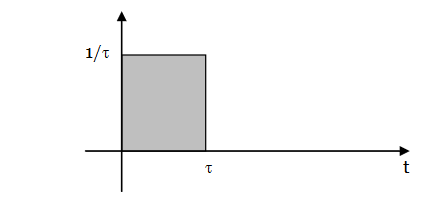
\includegraphics{../../../Imagenes/Superior/TransformadaDeLaplace/Laplace06.PNG}
	
	Sombreando bajo la curva obtenemos un rectangulo de area $\frac{1}{\tau} \cdot \tau = 1$.\\
	Al hacer que $\tau$ tienda a $0$ la base del rectangulo será infinitesimal y la altura infinita.
	
	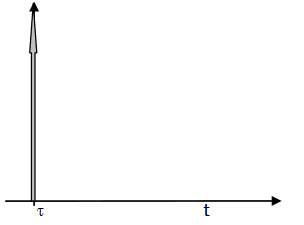
\includegraphics{../../../Imagenes/Superior/TransformadaDeLaplace/Laplace07.PNG}

Es decir, la función $\delta(t)$ es una función que vale $0$ en todo el eje real menos en $t = 0$ donde vale $+\infty$.\\
Matematicamente hablando $\delta(t)$ no es una función sino mas bien una distribución, pero aún así esta tiene una gran importancia y utilidad al momento de plantear y resolver modelos matematicos de sistemas fiscos y será tratada como una función. Para mas información buscar Delta de Dirac.

Algunas propiedades útiles de $\delta(t)$ son:
\\
\\
$a)$
$$
\int_{0}^{\infty} \delta(t) dt = 1
$$
\\
\\
$b)$
$$
\int_{0}^{\infty} \delta(t)f(t) dt = f(0)
$$
\\
\\
$c)$
$$
\int_{0}^{\infty} \delta(t-a)f(t) dt = f(a)
$$
\\
\\
\\

\huge Antitransformada de Laplace.
\normalsize
\\

Si $\exists \mathscr{L}[f(t)] = F(s) \Rightarrow f(t)$ es la antitransformada de $F(s)$.
\\
La antitransformada se indica: $$\mathscr{L}^{-1}[F(s)] = f(t)$$
Para el calculo de las antitransformadas se utiliza la tabla anterior pero esta vez en sentido inverso.
\\
\\
\Large Propiedades de la antitransformada de Laplace
\normalsize
\\
\\
$a)$ Linealidad
$$
\mathscr{L}^{-1}[F(s)] = f(t)\hspace{7pt} \wedge\hspace{7pt} \mathscr{L}^{-1}[G(s)] = g(t)\hspace{7pt} \wedge\hspace{7pt} k_{1} , k_{2} \in \mathbb{R} \Rightarrow \mathscr{L}^{-1}[k_{1}F(s) + k_{2}G(s)] = k_{1} f(t) + k_{2} g(t)
$$
\\
\\
$b)$ Primera propiedad de traslación
$$
f(t) = \mathscr{L}^{-1}[F(s)] \Rightarrow \mathscr{L}^{-1}[F(s-a)] = e^{at}f(t)
$$
\\
\\
$c)$ Segunda propiedad de traslación
$$ 
\mathscr{L}^{-1}[F(s)] = f(t) \hspace{5pt}
\Rightarrow \mathscr{L}^{-1}[e^{-as}F(s)] = g(t) = \left\{
	\begin{array}{ll}
		f(t-a) \hspace{10pt} t > a \\
		0 \hspace{40pt} t < a
	\end{array}
\right. \\ 
$$
\\
\\
$d)$ Cambio de escala
$$
f(t) = \mathscr{L}^{-1}[F(s)] \Rightarrow \mathscr{L}^{-1}[\frac{1}{a}F(\frac{s}{a})] = f(at) 	
$$
\\
\\
$e)$ Antitransformada de las derivadas
$$
f(t) = \mathscr{L}^{-1}[F(s)] \Rightarrow \mathscr{L}^{-1}[F^{(n)}(s)] = (-1)^{n}t^{n}f(t) 
$$
\\
\\
$f)$ Antitransformada de las integrales
$$
f(t) = \mathscr{L}^{-1}[F(s)] \Rightarrow \mathscr{L}^{-1}[\int_s^{\infty}F(u)du] =\frac{f(t)}{t}
$$
\\
\\
$g)$ Multiplicación por $s$
$$
f(t) = \mathscr{L}^{-1}[F(s)] \Rightarrow f(t) = \mathscr{L}^{-1}[sF(s)-f(0)] = f'(t) 
$$
\\
\\
$h)$ División por $s$
$$
f(t) = \mathscr{L}^{-1}[F(s)] \Rightarrow \mathscr{L}^{-1}[\frac{F(s)}{s}] = \int_0^{t} f(u)du
$$
\\
Para estudiar las propiedades de la antitransformada es importante tener en cuenta las de la transformada ya que son practicamete las mismas pero en sentido inverso. Es decir, multiplicar por $t$ es derivar en $s$ y multiplicar en $s$ es derivar en $t$. Todas las propiedaes de la transformada de Laplace (a exepción de las ultimas dos) tienen su contrapartida en la antitransformada. Veremos ahora un método para calcular ciertas antitransformadas que nos será útil.
\\
\\
\Large Resolución de antitransformada por fracciones simples.
\normalsize
\\
\\
Sea $F(s) = \frac{P(S)}{Q(S)}$ tal que el grado de $P(s) <$ grado de  $Q(s) \Rightarrow \frac{P(s)}{Q(s)}$ se puede escribir como una suma de fracciones simples del tipo:
\\Si $\alpha$ es raiz de $Q(s)$ con multiplicidad $p$:
$$ 
\frac{A}{(s-\alpha)^{p}}
$$
o bien si $Q(s)$ tiene raices complejas conjugadas:
$$
\frac{Bs+C}{s^{2}+bs+c}
$$
\\
Supongamos que debemos antitransformar la siguiente $F(s)$:
$$
F(s) = \frac{s+7}{s^{2}+6s+5}
$$
Primero factorizamos el denmoniador buscando sus raices, en este caso son $-1$ y $-5$.
$$
F(s) = \frac{s+7}{(s+1)(s+5)}
$$
Luego proponemos las constantes:
$$
F(s) = \frac{A}{s+1} + \frac{B}{s+5} = \frac{A(s+5)+B(s+1)}{s^{2}+6s+5}
$$
Podemos distribuir las constantes y por igualdad de polinomios armar un sistema de ecuaciones con la $F(s)$ del principio.
$$
A(s+5)+B(s+1) = s+7 \Rightarrow A+B = 1 \hspace{5pt} \wedge \hspace{5pt} 5A+B=7
$$
Resolvemos el sistema y encontramos:
$$
A = \frac{3}{2} \hspace{5pt} \wedge \hspace{5pt} B= -\frac{1}{2}
$$
Ahora reescribimos la $F(s)$ y estamos listos para antritransformar.
$$
F(s) = \frac{3}{2} \cdot\frac{1}{s+1} - \frac{1}{2} \cdot \frac{1}{s+5}
$$
Usando la tabla de transformadas y la propiedad de traslación nos queda:
$$
\mathscr{L}^{-1}[F(s)]  = \frac{3}{2} e^{-t} - \frac{1}{2} e^{-5t}
$$
\\
\\
\Large Resolución de ecuaciones diferenciales por trasnformada de Laplace
\normalsize
\\
\\
Dada una ecuación diferencial oridnaria, este metodo consiste en aplicar la transformada de Laplace lo cual la convierte en una ecuación algebraica. De este modo, se resuelve mas sencillamente en el dominio de Laplace y luego se antitransforma para volver a la variable original $t$.

Supongamos que debemos resolver la siguiente ecuacion diferencial con $y(0) = 0$ y $y'(0)=2$:
$$
y''(t) + 9y(t) = 0
$$
La idea de este metodo es no tener que resolver cuentas en el dominio del tiempo, por esto empezamos aplicando transformada de Laplace en ambos miembros:
$$
s^{2}Y(s)-sy(0)-y'(0)+9Y(s) = 0
$$
Si no se entiende de donde sale esta ecuacion volver a leer las propieades de la transformada de las derivadas.\\
Ahora reemplazamos los datos iniciales:
$$
s^{2}Y(s)-2+9Y(s) = 0
$$
Recordemos que nuestro objetivo es despejar la $Y(s)$ para así poder antitrasnformas y encontrar $y(t)$, para esto sacamos factor comun $Y(s)$:
$$
Y(s)(s^{2}+9) = 2 \Rightarrow Y(s) = \frac{2}{(s^{2}+9)}
$$
Antes de antritransformar, manipulamos algebraicamente para que la antitrasnformación sea mas sencilla:
$$
Y(s) = \frac{2}{(s^{2}+9)} = \frac{2}{3} \cdot  \frac{3}{(s^{2}+9)}
$$
Ahora antritransformamos:
$$
y(t) = \frac{2}{3} \sin(3t)
$$
No siempre la antritransformación será tan directa, muchas veces se debe aplicar fracciones simples para realizar este paso.
\\
\\
Supongamos que debemos resolver el siguiente sistema de ecuaciones difrenciales con $x(0)=8$ y $y(0)=3$:

	\begin{align}
		x'(t)  &= 2x(t)-3y(t) \\
		y'(t) &= y(t) -2x(t)
	\end{align}
\\
Empezaremos aplicando transformada de Laplace a ambas ecuaciones y reemplazando los datos iniciales:

\begin{align}
	sX(s)-8  &= 2X(s)-3Y(s) \\
	sY(s)-3 &= Y(s) -2X(s)
\end{align}

Vamos a utilizar el método de Cramer para la resolución, para ello, acomodamos los terminos:

\begin{align}
	(s-2)X(s) +3Y(s)&= 8 \\
	2X(s)+(s-1)Y(s) &= 3
\end{align}

Calculamos el determinante de la matriz de coeficientes:
$$
\Delta = \begin{vmatrix}
	s-2 & 3\\
	2 & s-1
	\end{vmatrix} = (s-2)(s-1) - 3\cdot 2 = s^{2}-3s+4  = (s-4)(s+1)
$$
Ahora calculamos el determinante asociado a la variable $X(s)$ es decir, en la columna de coeficientes de $X(s)$ reemplazamos con los terminos independientes originales.

$$
\Delta X(s)= \begin{vmatrix}
	8 & 3\\
	3 & s-1
	\end{vmatrix} = 8(s-1) - 3\cdot 3 = 8s-17
$$
Ahora por el metodo de cramer podemos escribir a $X(s)$ como:
$$
X(s) = \frac{8s-17}{(s-4)(s+1)}
$$
Ahora debemos antitransformar, para esto usamos fracciones simples:
$$
X(s) = \frac{A}{(s-4)} + \frac{B}{(s+1)}
$$
$$
A(s+1) + B(s-4) = 8s-17 \Rightarrow A+B = 8 \hspace{5pt} \wedge \hspace{5pt} A-4B = -17
$$
$$
A=3 \hspace{5pt} \wedge \hspace{5pt} B = 5
$$
Finalmente queda:
$$
X(s) = \frac{3}{(s-4)} + \frac{5}{(s+1)}
$$
Antitransformamos:
$$
x(t) = 3e^{4t} + 5e^{-t}
$$
Y ahora haremos lo mismo para $Y(s)$:

$$
\Delta Y(s)= \begin{vmatrix}
	s-2 & 8\\
	2 & 3
	\end{vmatrix} = (s-2)3 - 8\cdot 2 = 3s-22
$$
Ahora por el metodo de cramer podemos escribir a $Y(s)$ como:
$$
Y(s) = \frac{3s-22}{(s-4)(s+1)}
$$
Ahora debemos antitransformar, para esto usamos fracciones simples:
$$
Y(s) = \frac{A}{(s-4)} + \frac{B}{(s+1)}
$$
$$
A(s+1) + B(s-4) = 3s-22 \Rightarrow A+B = 3 \hspace{5pt} \wedge \hspace{5pt} A-4B = -22
$$
$$
A=-2 \hspace{5pt} \wedge \hspace{5pt} B = 5
$$
Finalmente queda:
$$
Y(s) = \frac{-2}{(s-4)} + \frac{5}{(s+1)}
$$
Antitransformamos:
$$
y(t) = -2e^{4t} + 5e^{-t}
$$
\\
\\
\Large Teorema de convolución o de Borel.
\normalsize
\\
\\
$$
\mathscr{L}^{-1}[F(s)] = f(t) \hspace{3pt} \wedge \hspace{3pt} \Rightarrow \mathscr{L}^{-1}[F(s)\cdot G(s)] = \int_{0}^{t}f(u) g(t-u)du
$$
Observar que este teorema tambien significa que: 
$$
F(s)\cdot G(s) =\mathscr{L}[ \int_{0}^{t}f(u) g(t-u)du]
$$
Es un teorema util para resolver ecuaciones diferenciales de convolucion pero no le daremos mucho detalle, se tratará casi como una propiedad.




\end{document}